%	-------------------------------------------------------------------------------
%
%
%
%
%
%
%
%
%	-------------------------------------------------------------------------------

%	\documentclass[10pt,xcolor=pdftex,dvipsnames,table]{beamer}
%	16:10
%	\documentclass[ aspectratio=1610, 10pt,blue,xcolor=pdftex,dvipsnames,table,handout]{beamer}
%	\documentclass[ aspectratio=1610, 10pt,blue,xcolor=pdftex,dvipsnames,table,handout,notes]{beamer}
%	16:9 
%	\documentclass[ aspectratio=169,  10pt,blue,xcolor=pdftex,dvipsnames,table,handout]{beamer}
	\documentclass[ aspectratio=169,  12pt,blue,xcolor=pdftex,dvipsnames,table,handout,notes]{beamer}
%	14:9 
%	\documentclass[ aspectratio=149,  10pt,blue,xcolor=pdftex,dvipsnames,table,handout]{beamer}
%	5:4
%	\documentclass[ aspectratio=54,   10pt,blue,xcolor=pdftex,dvipsnames,table,handout]{beamer}
%	4:3 default
%	\documentclass[ aspectratio=43, 10pt,blue,xcolor=pdftex,dvipsnames,table,handout]{beamer}
%	3:2 
% 	\documentclass[ aspectratio=32, 10pt,blue,xcolor=pdftex,dvipsnames,table,handout]{beamer}







		% Font Size
		%	default font size : 11 pt
		%	8,9,10,11,12,14,17,20
		%
		% 	put frame titles 
		% 		1) 	slideatop
		%		2) 	slide centered
		%
		%	navigation bar
		% 		1)	compress
		%		2)	uncompressed
		%
		%	Color
		%		1) blue
		%		2) red
		%		3) brown
		%		4) black and white	
		%
		%	Output
		%		1)  	[default]	
		%		2)	[handout]		for PDF handouts
		%		3) 	[trans]		for PDF transparency
		%		4)	[notes=hide/show/only]

		%	Text and Math Font
		% 		1)	[sans]
		% 		2)	[sefif]
		%		3) 	[mathsans]
		%		4)	[mathserif]


		%	---------------------------------------------------------	
		%	슬라이드 크기 설정 ( 128mm X 96mm )
		%	---------------------------------------------------------	
			\setbeamersize{text margin left=10mm}
			\setbeamersize{text margin right=10mm}

%			% Format presentation size to A4
%			\usepackage[size=a4]{beamerposter}		% A4용지 크기 사용

%			% Format presentation size to A4
%			\setlength{\paperwidth}{297mm}
%			\setlength{\paperheight}{210mm}
%			\setlength{\textwidth}{287mm}
%			\setlength{\textheight}{200mm}   

%			% Format presentation size to A4 길게
			\setlength{\paperwidth}	{210mm}
			\setlength{\paperheight}	{297mm}
			\setlength{\textwidth}		{190mm}
			\setlength{\textheight}	{287mm}   


	%	========================================================== 	Package
			\usepackage{kotex}						% 한글 사용
			\usepackage{amssymb,amsfonts,amsmath}	% 수학 수식 사용
			\usepackage{color}					%
			\usepackage{colortbl}					%

			\usepackage{tikz}				% TikZ picture
			\usepackage{keycommand}
			\usetikzlibrary{shapes,arrows,positioning}
			\usetikzlibrary{shadows}

			\usepackage{tikzscale}
			\usepackage{adjustbox}

			\usepackage{pgfgantt}  		% 간트 챠트 입력용 패키지




		
		%	---------------------------------------------------------	
		%		유인물 출력 : 출력할대 조정해서 출력 할것
		%	---------------------------------------------------------	

			\usepackage{pgfpages}
%			\pgfpagesuselayout{2 on 1}[letterpaper]
%			\pgfpagesuselayout{4 on 1}[letterpaper]
%			\pgfpagesuselayout{8 on 1}[letterpaper]

%			\pgfpagesuselayout{resize to}[a4paper,landscape,border shrink=5mm]
			\pgfpagesuselayout{resize to}[a4paper, border shrink=5mm]
%			\pgfpagesuselayout{resize to}[a4paper,border shrink=5mm]
%			\pgfpagesuselayout{2 on 1}[a4paper,border shrink=5mm]
%			----------------------------------------------------- 출력 시 설정	1
%			\pgfpagesuselayout{2 on 1}[a4paper]
%			\usecolortheme{seagull}	% 휜색
%			----------------------------------------------------- 출력 시 설정	2
%			\pgfpagesuselayout{2 on 1}[a4paper,border shrink=5mm]
%			\usecolortheme{dove}
%			----------------------------------------------------- 
%			\pgfpagesuselayout{4 on 1}[a4paper,border shrink=5mm]
%			\pgfpagesuselayout{8 on 1}[a4paper,border shrink=5mm]


	%		========================================================= 	Theme

		%	---------------------------------------------------------	
		%	전체 테마
		%	---------------------------------------------------------	
		%	테마 명명의 관례 : 도시 이름
%			\usetheme{default}			%
%			\usetheme{Madrid}    		%
%			\usetheme{CambridgeUS}    	% -red, no navigation bar
			\usetheme{Antibes}			% -blueish, tree-like navigation bar

		%	----------------- table of contents in sidebar
%			\usetheme{Berkeley}		% -blueish, table of contents in sidebar
									% 개인적으로 마음에 듬
%			\usetheme{Marburg}			% - sidebar on the right
%			\usetheme{Hannover}		% 왼쪽에 마크
%			\usetheme{Berlin}			% - navigation bar in the headline
%			\usetheme{Szeged}			% - navigation bar in the headline, horizontal lines
%			\usetheme{Malmoe}			% - section/subsection in the headline

%			\usetheme{Singapore}
%			\usetheme{Amsterdam}

		%	---------------------------------------------------------	
		%	색 테마
		%	---------------------------------------------------------	
%			\usecolortheme{albatross}	% 바탕 파란
%			\usecolortheme{crane}		% 전체적으로 노란색 계열
%			\usecolortheme{beetle}		% 바탕 회색
%			\usecolortheme{dove}		% 전체적으로 흰색 ( 출력용으로 적합 : 잉크 절약)
%			\usecolortheme{fly}		% 전체적으로 회색
%			\usecolortheme{seagull}	% 휜색
%			\usecolortheme{wolverine}	& 제목이 노란색
%			\usecolortheme{beaver}

		%	---------------------------------------------------------	
		%	Inner Color Theme 			내부 색 테마 ( 블록의 색 )
		%	---------------------------------------------------------	

%			\usecolortheme{rose}		% 흰색
%			\usecolortheme{lily}		% 색 안 칠한다
%			\usecolortheme{orchid} 	% 진하게

		%	---------------------------------------------------------	
		%	Outter Color Theme 		외부 색 테마 ( 머리말, 고리말, 사이드바 )
		%	---------------------------------------------------------	

%			\usecolortheme{whale}		% 진하다
%			\usecolortheme{dolphin}	% 중간
%			\usecolortheme{seahorse}	% 연하다

		%	---------------------------------------------------------	
		%	Font Theme 				폰트 테마
		%	---------------------------------------------------------	
%			\usfonttheme{default}		
			\usefonttheme{serif}			
%			\usefonttheme{structurebold}			
%			\usefonttheme{structureitalicserif}			
%			\usefonttheme{structuresmallcapsserif}			



		%	---------------------------------------------------------	
		%	Inner Theme 				
		%	---------------------------------------------------------	

%			\useinnertheme{default}
			\useinnertheme{circles}		% 원문자			
%			\useinnertheme{rectangles}		% 사각문자			
%			\useinnertheme{rounded}			% 깨어짐
%			\useinnertheme{inmargin}			




		%	---------------------------------------------------------	
		%	이동 단추 삭제
		%	---------------------------------------------------------	
%			\setbeamertemplate{navigation symbols}{}

		%	---------------------------------------------------------	
		%	문서 정보 표시 꼬리말 적용
		%	---------------------------------------------------------	
%			\useoutertheme{infolines}


			
	%	---------------------------------------------------------- 	배경이미지 지정
%			\pgfdeclareimage[width=\paperwidth,height=\paperheight]{bgimage}{./fig/Chrysanthemum.jpg}
%			\setbeamertemplate{background canvas}{\pgfuseimage{bgimage}}

		%	---------------------------------------------------------	
		% 	본문 글꼴색 지정
		%	---------------------------------------------------------	
%			\setbeamercolor{normal text}{fg=purple}
%			\setbeamercolor{normal text}{fg=red!80}	% 숫자는 투명도 표시


		%	---------------------------------------------------------	
		%	itemize 모양 설정
		%	---------------------------------------------------------	
%			\setbeamertemplate{items}[ball]
%			\setbeamertemplate{items}[circle]
%			\setbeamertemplate{items}[rectangle]


		%	---------------------------------------------------------	
		%	상자 모양새 설정
		%	---------------------------------------------------------	
%			\setbeamertemplate{blocks}[rounded,shadow=true]
%			\begin{block}
%			\begin{theorem}
%			\begin{lemma}
%			\begin{proof}
%			\begin{corollary}
%			\begin{example}
%			\begin{exampleblock}
%			\begin{alertblock}




		\setbeamercovered{dynamic}


		%	---------------------------------------------------------	
		%		Background 
		%	---------------------------------------------------------	

%			\beamersetaveragebackground{yellow!20}
%			\beamertemplatesolidbackgroundcolor{yellow!20}
%			\beamertemplategridbackground [5mm]




		% --------------------------------- 	문서 기본 사항 설정
		\setcounter{secnumdepth}{1} 		% 문단 번호 깊이
		\setcounter{tocdepth}{1} 			% 문단 번호 깊이





























% ------------------------------------------------------------------------------
% Begin document (Content goes below)
% ------------------------------------------------------------------------------
	\begin{document}
	

			\title{gantt Chart}
			\subtitle{사용설명서}
			\author{김대희}
			\date[2011.11.10]{2015년 1월}
			\institute[KTS]{(주)서영엔지니어링 \texttt{http://symsone.seoyeong.co.kr/}}



	%	==========================================================
	%		타이틀 페이지 출력
	%	----------------------------------------------------------
		\begin{frame}[plain]
		\titlepage
		\end{frame}




	%	==========================================================
	%		목차
	%	----------------------------------------------------------
%		\begin{frame}[plain]
%		\frametitle{목차}
%		\note[item]{목차 내용의 출력}
%
%		\tableofcontents
%
%
%		\end{frame}





	%	==========================================================
	%		예제 : 선의 두께
	%	----------------------------------------------------------
		\begin{frame}[t]
		\frametitle{Titles}


		\begin{block}


	% -------------------------------------
			\begin{ganttchart}[	hgrid, 
								vgrid,
%								inline
								x unit=0.8cm,
								y unit chart=0.6cm,
								y unit title=0.8cm,
							]{1}{12}
			% -------------------------------------
			\gantttitle{야간 작업 일정}{12} \\
			\gantttitlelist{6,7,8,9,10,11,12,01,02,03,04,05}{1} \\
			% -------------------------------------
			\ganttbar{안전 헨스 설치}	{ 2}{ 2} \\
			\ganttgroup{굴착}{2}{7} \\
			\ganttbar{컷팅}			{ 2}{ 3} \\
			\ganttbar{포장 깨기}		{ 3}{ 4} \\
			\ganttbar{초기 굴착}		{ 5}{ 5} \\
			\ganttbar{흙막이 설치}		{ 6}{ 6} \\
			\ganttbar{최종 굴착}		{ 7}{ 7} \\

			\ganttgroup{관부설}		{ 3}{ 8} \\
			\ganttbar{관 부설}			{ 3}{ 8} \\

			\ganttgroup{되메우기 및 포장}	{ 9}{12} \\
			\ganttbar{모래 되메우기}		{ 9}{ 9} \\
			\ganttbar{토사 되메우기}		{ 9}{10} \\
			\ganttbar{보조기층}			{11}{11} \\
			\ganttbar{택 코팅}				{13}{13} \\
			\ganttbar{기층}				{13}{13} \\
			\ganttbar{안전 헨스 철거}		{12}{12} \\

			\end{ganttchart}

		\end{block}
		\end{frame}

	%	==========================================================
	%		The Canvas
	%	----------------------------------------------------------
		\begin{frame}[t]
		\frametitle{The Canvas}

			The ganttchart environment draws a single Gantt chart\\

			\textbackslash begin\{ganttchart\}[\(<\)options\(>\)]
										\{\(<\)start tss\(>\)\}
										\{\(<\)end tss\(>\)\}\\
			.......\\
			\textbackslash end\{ganttchart\}


		\begin{description}
		\item[options]
		\item[start tss]
		\item[end tss]
		\end{description}

		\end{frame}




	%	==========================================================
	%		Chart의 높이와 폭
	%	----------------------------------------------------------
		\begin{frame}[t]
		\frametitle{Chart의 높이와 폭}

		\begin{enumerate}
		\item[]	x unit = \(<\) dimension \(>\) .5cm
		\item[]	y unit title = \(<\) dimension \(>\)  1cm
		\item[]	y unit chart = \(<\) dimension \(>\)  1cm
		\end{enumerate}

		\begin{block}{Chart의 높이와 폭}
			\textbackslash begin\{ganttchart\}[ \\
			\hspace {4em} x unit=1cm, \\
			\hspace {4em} y unit title=.6cm, \\
			\hspace {4em} y unit chart=1.5cm \\
			\hspace {4em} ]\{1\}\{6\} \\
			\hspace {2em} \textbackslash gantttitle\{Title 1\}\{6\} \textbackslash \textbackslash \\
			\hspace {2em} \textbackslash gantttitle\{Title 2\}\{6\} \textbackslash \textbackslash \\
			\hspace {2em} \textbackslash ganttbar\{\}\{1\}\{3\} \textbackslash \textbackslash \\
			\hspace {2em} \textbackslash ganttbar\{\}\{4\}\{6\} \\
			\textbackslash end\{ganttchart\} \\
		\end{block}
	
			\begin{ganttchart}[
			x unit=1cm,
			y unit title=.6cm,
			y unit chart=1.5cm
			]{1}{6}
			\gantttitle{Title 1}{6} \\
			\gantttitle{Title 2}{6} \\
			\ganttbar{}{1}{3} \\
			\ganttbar{}{4}{6}
			\end{ganttchart}
		\end{frame}




	%	==========================================================
	%		Chart grid
	%	----------------------------------------------------------
		\begin{frame}[t]
		\frametitle{Chart grid}

		\begin{enumerate}
		\item[]	hgrid [=false or true or \(<\)style list\(>\)]
		\item[]	hgrid style /.style=\(<\)style\(>\)
		\item[]	vgrid [=false or true or \(<\) style list \(>\)]
		\end{enumerate}



		\begin{ganttchart}[		hgrid=true,
								vgrid={*2{red},*1{white},*{10}{blue, dashed}}	,
						]{1}{20}
		\gantttitle{Title 1}{20} \\
		\ganttbar{}{1}{8} \\
		\ganttbar{}{9}{20}
		\end{ganttchart}



		\end{frame}


	%	==========================================================
	%		Chart grid : Today
	%	----------------------------------------------------------
		\begin{frame}[t]
		\frametitle{Chart grid : Today}

		\begin{enumerate}
		\item[]	hgrid [=false or true or \(<\)style list\(>\)]
		\item[]	hgrid style /.style=\(<\)style\(>\)
		\item[]	vgrid [=false or true or \(<\) style list \(>\)]
		\end{enumerate}



		\begin{ganttchart}[		hgrid=true,
								vgrid={*2{red},*1{white},*{10}{blue, dashed}}	,
								today=2
						]{1}{20}
		\gantttitle{Title 1}{20} \\
		\ganttbar{}{1}{8} \\
		\ganttbar{}{9}{20}
		\end{ganttchart}



		\end{frame}









	%	==========================================================
	%		Titles
	%	----------------------------------------------------------
		\begin{frame}[t]
		\frametitle{Titles}

%		\begin{block}
%		\end{block}


		\end{frame}


	%	==========================================================
	%		Predefined Chart Elements
	%	----------------------------------------------------------
		\begin{frame}[t]
		\frametitle{Predefined Chart Elements}


		\end{frame}


	%	==========================================================
	%		Options : Chart Element Appearance
	%	----------------------------------------------------------
		\begin{frame}[t]
		\frametitle{Options : Chart Element Appearance}


		\begin{ganttchart}[vgrid, hgrid, bar/.style={fill=red!50}]{1}{12}
			\gantttitle{Title}{12} \\
			\ganttbar									{Task 1}{1}{3} \\
			\ganttbar[bar/.style={fill=yellow, dashed}]	{Task 2}{4}{10} \\
			\ganttbar[bar/.style={fill=green, draw=none}]	{Final task}{11}{12}
		\end{ganttchart}

\vskip 2cm

		\begin{ganttchart}
			[vgrid, hgrid]{1}{12}
			\gantttitle{Title}{12} \\
			\ganttbar[bar label node/.style={left=2cm}]	{Task 1}{1}{3} \\
			\ganttbar[bar label font=\color{orange}]		{Task 2}{4}{10} \\
			\ganttbar[]								{Final task}{11}{12}
		\end{ganttchart}

\vskip 2cm

		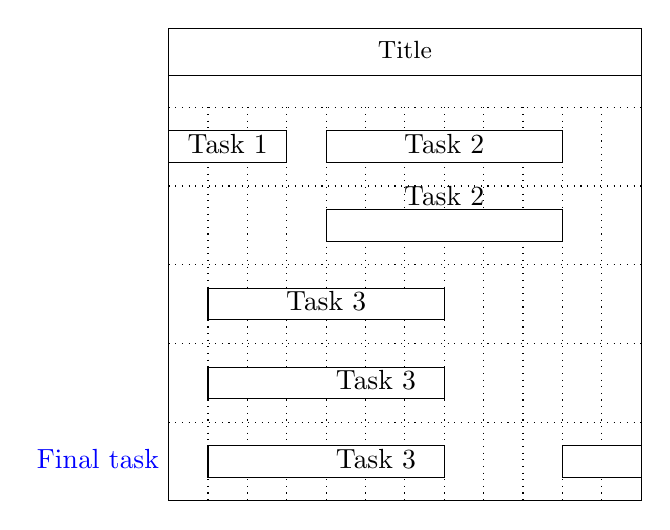
\begin{tikzpicture}
		\begin{ganttchart}[vgrid, hgrid, inline]{1}{12}
			\gantttitle{Title}{12} \\
			\ganttbar										{Task 1}{1}{3}
			\ganttset{bar label inline anchor node/.style=above}
			\ganttbar										{Task 2}{5}{10} \\
			\ganttbar[bar inline label node/.style=above]	{Task 2}{5}{10} \\
			\ganttbar[bar label inline node/.style=right]	{Task 3}{2}{7}\\
			\ganttbar[bar inline label node/.style=right]	{Task 3}{2}{7}\\
			\ganttset{bar label font=\color{blue}}
			\ganttbar{Task 3}{2}{7}
			\ganttbar[bar inline label node/.style=right]	{Task 3}{2}{7}
			\ganttbar[inline=false]						{Final task}{11}{12}
		\end{ganttchart}
		\end{tikzpicture}

		\end{frame}




	%	==========================================================
	%		Options : Label Formatting
	%	----------------------------------------------------------
		\begin{frame}[t]
		\frametitle{Options : Label Formatting}



		\end{frame}


	%	==========================================================
	%		Options : Chart Element Positioning
	%	----------------------------------------------------------
		\begin{frame}[t]
		\frametitle{Options : Chart Element Positioning}

%		\begin{block}
%		\end{block}


		\end{frame}


	%	==========================================================
	%		Options : Progress
	%	----------------------------------------------------------
		\begin{frame}[t]
		\frametitle{Options : Progress}

%		\begin{block}
%		\end{block}


		\end{frame}



	%	==========================================================
	%		New Node Shapes
	%	----------------------------------------------------------
		\begin{frame}[t]
		\frametitle{New Node Shapes}

%		\begin{block}
%		\end{block}


		\end{frame}

	%	==========================================================
	%		Defining Custom Chart Elements
	%	----------------------------------------------------------
		\begin{frame}[t]
		\frametitle{Defining Custom Chart Elements}

%		\begin{block}
%		\end{block}


		\end{frame}



	%	==========================================================
	%		Links
	%	----------------------------------------------------------
		\begin{frame}[t]
		\frametitle{Links}

%		\begin{block}
%		\end{block}


		\end{frame}























% ------------------------------------------------------------------------------
% End document
% ------------------------------------------------------------------------------
\end{document}


